%!LW recipe=xelatex
\documentclass[aspectratio=169]{beamer}

\usepackage{tikz}

\usepackage{tikz-network}
\usepackage{tikz-cd}
\usepackage{tikzit}
\usepackage{subcaption}
\usepackage{minted}
\usepackage{mathtools}
\usepackage{stmaryrd}
\newcommand{\consistency}{{\smile}}
\usepackage{adjustbox}
\usepackage{appendixnumberbeamer}

\usepackage[style=authoryear,backend=bibtex]{biblatex} % or backend=biber
\addbibresource{../../bibliography.bib}

% \hypersetup{
%     colorlinks=true,
%     linkcolor=gray,
%     filecolor=magenta,      
%     urlcolor=cyan,
%     pdftitle={Overleaf Example},
%     pdfpagemode=FullScreen,
%     }

\input{../../sample.tikzstyles}
\input{../../hypergraph.tikzstyles}
\input{../../hypergraph.tikzdefs}

\usetheme[subsectionpage=simple]{metropolis}
% \usetheme{awesome}

% \setsansfont{Ubuntu}
% \setmonofont{Ubuntu Mono}


\setbeamertemplate{footline}
{
  \leavevmode
  \hbox{
  \begin{beamercolorbox}[wd=.15\paperwidth,ht=2.25ex,dp=1ex,center]{title in head/foot}
    \usebeamerfont{author in head/foot}\insertshortauthor
  \end{beamercolorbox}

  \begin{beamercolorbox}[wd=.7\paperwidth,ht=2.25ex,dp=1ex,center]{author in head/foot}
    \usebeamerfont{author in head/foot}\insertshorttitle
  \end{beamercolorbox}

  \begin{beamercolorbox}[wd=.15\paperwidth,ht=2.25ex,dp=1ex,center]{title in head/foot}
    \insertframenumber{} / \inserttotalframenumber
  \end{beamercolorbox}
  }
}

\makeatletter
\metropolis@disablesubsectionpage
\makeatother

\newcommand{\bsubsection}[1]{\subsection{$\bullet$ #1}}

\title{Equivalence Hypergraphs: DPO Rewriting for Monoidal E-Graphs} 
\date{LICS, 2025} % Use metropolis theme 
\author[Aleksei Tiurin]{$\textbf{Aleksei Tiurin}^{\dagger}$,$\text{Chris Barrett}^{\dagger}$,$\text{Dan R. Ghica}^{\dagger,\ddagger}$, $\text{Nick Hu}^{\dagger}$}
\institute{$^{\dagger}$University of Birmingham, $^{\ddagger}$Huawei Central Software Institute}
\begin{document} 


\renewcommand{\maketitle}{
  \begin{frame}[plain]
    \begin{minipage}[c]{0.75\textwidth}
      \usebeamerfont{title}\usebeamercolor[fg]{title}\inserttitle\par
      \ifx\insertsubtitle\@empty\else
        \vskip0.5em
        \usebeamerfont{subtitle}\usebeamercolor[fg]{subtitle}\insertsubtitle\par
      \fi
      \vskip1em
      \usebeamerfont{author}\insertauthor\par
      \usebeamerfont{institute}\insertinstitute\par
      \usebeamerfont{date}\insertdate\par
      \alert{\rule{\textwidth}{1.5pt}}
    \end{minipage}%
    \hfill
    \begin{minipage}[c]{0.2\textwidth}
      
\includegraphics[width=\linewidth]{figures/birmingham_logo} % your logo file here
    \end{minipage}
  \end{frame}
}

\maketitle 

% \begin{frame}{Table of contents}
%     \small
%     \setbeamertemplate{section in toc}[sections numbered]
%     \tableofcontents
% \end{frame}

\section{What and Why?}
\bsubsection{E-graphs}

\begin{frame}{E-graphs}
    Data structure to \alert{efficiently} represent an equivalence relation on a set of terms over an \alert{algebraic} signature $\Sigma$
    \pause
    \begin{itemize}
        \item $\Sigma_{\mathbf{Mon}} = \{\mathbb{S},\mu : 2 \to 1, i: 0 \to 1\}$
        \item $i$, $\mu(s_1,s_2), s_i \in \mathbb{S}$, $\ldots$
    \end{itemize}
    \pause
    \vfill
    The relation is refined by applying equations \alert{non-destructively}, \alert{saturating} the e-graph
    \begin{itemize}
        \item Solves \emph{phase ordering} problem
        \item $\mu(x,i) \equiv x$, $\mu(x,y) \equiv \mu(y,x)$, $\ldots$
    \end{itemize}
    \vfill
\end{frame}
\begin{frame}{E-graphs}
    \vfill
    Once saturated, the \alert{best} candidate can be extracted from the set
    \vfill
    \pause
    The \alert{best} candidate is domain-specific
    \begin{itemize}
        \item Best program in compiler optimisation
        \item Smallest test-case in fuzzy testing
        \item Smallest digital circuit
        \item $\ldots$
    \end{itemize}
    \vfill
    \pause
    Or, the saturated e-graph can be used to check if two terms are equivalent
    \begin{itemize}
        \item Tactics for proof assistants
    \end{itemize}
    \pause
    \vfill\
    Many more applications are proposed at EGRAPHS workshop annually
    % However, there are more general theories that describe the interaction of processes, \textit{e.g.}, quantum
\end{frame}

\bsubsection{Monoidal theories}

\begin{frame}{E-graphs}
\begin{minipage}{0.45\linewidth}
E-classes $\scalebox{0.4}{\begin{tikzpicture}\begin{pgfonlayer}{nodelayer}\node [style=empty diag red] (0) at (0, 0) {};\end{pgfonlayer}\end{tikzpicture}}$,$\scalebox{0.4}{\begin{tikzpicture}\begin{pgfonlayer}{nodelayer}\node [style=empty diag yellow] (0) at (0, 0) {};\end{pgfonlayer}\end{tikzpicture}}$,$\scalebox{0.4}{\begin{tikzpicture}\begin{pgfonlayer}{nodelayer}\node [style=empty diag blue] (0) at (0, 0) {};\end{pgfonlayer}\end{tikzpicture}}$,$\scalebox{0.4}{\begin{tikzpicture}\begin{pgfonlayer}{nodelayer}\node [style=empty diag green] (0) at (0, 0) {};\end{pgfonlayer}\end{tikzpicture}}$,$\scalebox{0.4}{\begin{tikzpicture}\begin{pgfonlayer}{nodelayer}\node [style=empty diag black] (0) at (0, 0) {};\end{pgfonlayer}\end{tikzpicture}}$,$\ldots$ 
\begin{itemize}
    \item Set of equivalent terms represented by enodes rooted at this particular e-class
\end{itemize}
\vfill
E-nodes $\begin{tikzpicture}\begin{pgfonlayer}{nodelayer}\node [style=round box] (0) at (0, 0) {$f_1$};\node [style=none] (1) at (-0.5, -0.5) {};\node [style=none] (2) at (0.5, -0.5) {};\node [style=none] (3) at (0, -0.5) {$\small\ldots$};\end{pgfonlayer}\begin{pgfonlayer}{edgelayer}\draw [style=new edge style 1] (0.center) to (1.center);\draw [style=new edge style 1] (0.center) to (2.center);\end{pgfonlayer}\end{tikzpicture}$, $\ldots$, $\begin{tikzpicture}\begin{pgfonlayer}{nodelayer}\node [style=round box] (0) at (0, 0) {$f_n$};\node [style=none] (1) at (-0.5, -0.5) {};\node [style=none] (2) at (0.5, -0.5) {};\node [style=none] (3) at (0, -0.5) {$\small\ldots$};\end{pgfonlayer}\begin{pgfonlayer}{edgelayer}\draw [style=new edge style 1] (0.center) to (1.center);\draw [style=new edge style 1] (0.center) to (2.center);\end{pgfonlayer}\end{tikzpicture}$
\begin{itemize}
    \item A component of an e-class
\end{itemize}
\vfill
Machinery to maintain \alert{sharing} and \alert{congruence} ($t_1 \cong t_2 \implies f\;(t_1) \cong f\;(t_2)$)
\begin{itemize}
    \item Union-find
    \item Hashconsing
\end{itemize}
\end{minipage}
\hfill
\begin{minipage}{0.45\linewidth}
\[
\tikzfig{./figures/e-graph-generic-example}
\]
\end{minipage}
\end{frame}

\begin{frame}{E-graphs}
\begin{example}[$(a * 2) / 2$]
    \[
    \tikzfig{./figures/e-graph-example-a-no-label}
    \]
\end{example}
\end{frame}

\begin{frame}{E-graphs}
    \begin{example}[$x * 2 \to x <\!\!< 1$]
        \hspace{-3em}
        \begin{minipage}{0.25\linewidth}
        \[
        \scalebox{0.8}{
        \tikzfig{./figures/e-graph-example-a-no-label}
        }
        \]    
        \end{minipage}
        \pause
        \hspace{-1.5em}
        \begin{minipage}{0.075\linewidth}
        \[
        \xRightarrow{\texttt{add}(a <\!\!< 1)}
        \]
        \end{minipage}
        \hfill
        \begin{minipage}{0.25\linewidth}
            \[
            \scalebox{0.8}{
            \tikzfig{./figures/e-graph-example-b-add}
            }
            \]    
        \end{minipage}
        \hfill
        \pause
        \begin{minipage}{0.1\linewidth}
            \[
            \xRightarrow{\texttt{merge}(\scalebox{0.3}{\begin{tikzpicture}\begin{pgfonlayer}{nodelayer}\node [style=empty diag yellow] (0) at (0, 0) {<\!\!<};\end{pgfonlayer}\end{tikzpicture}},\scalebox{0.3}{\begin{tikzpicture}\begin{pgfonlayer}{nodelayer}\node [style=empty diag black] (0) at (0, 0) {*};\end{pgfonlayer}\end{tikzpicture}})}
            \]
        \end{minipage}
        \hfill
        \begin{minipage}{0.25\linewidth}
            \[
            \scalebox{0.8}{
            \tikzfig{./figures/e-graph-example-b-merged}
            }
            \]
        \end{minipage}
        \hfill
    \end{example}
\end{frame}


\begin{frame}{E-graphs}
    \begin{example}[$(x * y) / z \to x * (y / z)$]
        \hspace{-2.5em}
        \begin{minipage}{0.25\linewidth}
        \[
        \scalebox{0.8}{
        \tikzfig{./figures/e-graph-example-b-merged}
        }
        \]    
        \end{minipage}
        \pause
        \hspace{-1.5em}
        \begin{minipage}{0.075\linewidth}
        \[
        \xRightarrow{\texttt{add}(a * (2/2))}
        \]
        \end{minipage}
        \hfill
        \begin{minipage}{0.25\linewidth}
            \[
            \scalebox{0.8}{
                \tikzfig{./figures/e-graph-example-c-add}
            }
            \]    
        \end{minipage}
        \hfill
        \pause
        \begin{minipage}{0.1\linewidth}
            \[
            \xRightarrow{\texttt{merge}(\scalebox{0.3}{\begin{tikzpicture}\begin{pgfonlayer}{nodelayer}\node [style=empty diag yellow] (0) at (0, 0) {/};\end{pgfonlayer}\end{tikzpicture}},\scalebox{0.3}{\begin{tikzpicture}\begin{pgfonlayer}{nodelayer}\node [style=empty diag black] (0) at (0, 0) {*};\end{pgfonlayer}\end{tikzpicture}})}
            \]
        \end{minipage}
        \hfill
        \begin{minipage}{0.25\linewidth}
            \[
            \scalebox{0.8}{
            \tikzfig{./figures/e-graph-example-c-merged}
            }
            \]
        \end{minipage}
        \hfill
    \end{example}
\end{frame}


\begin{frame}{E-graphs}
    \begin{example}[$(x / x) \to 1$]
        \hspace{-2.5em}
        \begin{minipage}{0.25\linewidth}
        \[
        \scalebox{0.8}{
        \tikzfig{./figures/e-graph-example-c-merged}
        }
        \]    
        \end{minipage}
        \pause
        \hfill
        \begin{minipage}{0.075\linewidth}
        \[
        \xRightarrow{\texttt{add}(1)}
        \]
        \end{minipage}
        \hfill
        \begin{minipage}{0.25\linewidth}
            \[
            \scalebox{0.8}{
            \tikzfig{./figures/e-graph-example-c-merged}
            }
            \]    
        \end{minipage}
        \hfill
        \pause
        \begin{minipage}{0.1\linewidth}
            \[
            \xRightarrow{\texttt{merge}(\scalebox{0.3}{\begin{tikzpicture}\begin{pgfonlayer}{nodelayer}\node [style=empty diag black] (0) at (0, 0) {/};\end{pgfonlayer}\end{tikzpicture}},\scalebox{0.3}{\begin{tikzpicture}\begin{pgfonlayer}{nodelayer}\node [style=empty diag black] (0) at (0, 0) {1};\end{pgfonlayer}\end{tikzpicture}})}
            \]
        \end{minipage}
        \hfill
        \begin{minipage}{0.25\linewidth}
            \[
            \scalebox{0.8}{
            \tikzfig{./figures/e-graph-example-d-merged}
            }
            \]
        \end{minipage}
        \hfill
    \end{example}
\end{frame}


\begin{frame}{E-graphs}
    \begin{example}[$x * 1 \to x$]
        \hspace{-2em}
        % \hfill
        \begin{minipage}{0.2\linewidth}
        \[
        \scalebox{0.8}{
        \tikzfig{./figures/e-graph-example-d-merged}
        }
        \]    
        \end{minipage}
        \pause
        \hspace{2em}
        \begin{minipage}{0.1\linewidth}
        \[
        \xRightarrow{\texttt{add}(a)}
        \]
        \end{minipage}
        \begin{minipage}{0.2\linewidth}
            \[
            \scalebox{0.8}{
            \tikzfig{./figures/e-graph-example-d-merged}
            }
            \]    
        \end{minipage}
        \hspace{1em}
        \pause
        \begin{minipage}{0.25\linewidth}
            \[
            \xRightarrow{\texttt{merge}(\scalebox{0.3}{\begin{tikzpicture}\begin{pgfonlayer}{nodelayer}\node [style=empty diag black] (0) at (0, 0) {/\;,*};\end{pgfonlayer}\end{tikzpicture}},\scalebox{0.3}{\begin{tikzpicture}\begin{pgfonlayer}{nodelayer}\node [style=empty diag black] (0) at (0, 0) {a};\end{pgfonlayer}\end{tikzpicture}})}
            \]
        \end{minipage}
        \hspace{-2em}
        \begin{minipage}{0.2\linewidth}
            \[
            \scalebox{0.8}{
            \tikzfig{./figures/e-graph-example-e-merged}
            }
            \]
        \end{minipage}
    \end{example}
\end{frame}


\begin{frame}{What we do}
We introduce \alert{categorical semantics} for e-graphs which has the following benefits
\begin{itemize}
    \item Provides new perspective on e-graph operations
    \item Opens up new avenues for applications
\end{itemize}
\end{frame}

\begin{frame}{Categorical semantics}

We generalise from \alert{algebraic} signatures to arbitrary \alert{monoidal signatures}
\begin{itemize}
    \item $\Sigma_{\mathbf{CMon}} = \{\mathbb{S},\mu : 1 \to 2, i : 1 \to 0\}$
\end{itemize}
These induce corresponding syntactic categories $\mathbf{S}(\Sigma)$ (\textbf{PROP}s)
\begin{itemize}
    \item Morphisms are given by terms freely constructed using functional symbols from $\Sigma$ and $\otimes,\; ;, \textsf{sym}, id$ quotiented by the axioms of symmetric monoidal categories
\end{itemize}

We can also consider equations between $\Sigma$-terms $\mathcal{E}$, i.e. pairs of morphisms $(l,r)$ with matching arities and co-arities (types), which gives rise to $\mathbf{SMT}(\Sigma,\mathcal{E})$ and the corresponding syntactic category $\mathbf{S}(\Sigma, \mathcal{E})$, where morphisms are additionally quotiented by $\mathcal{E}$
\begin{itemize}
    \item $\mathcal{E} = \{(\mu(x);id \otimes i \equiv x), \ldots\}$
\end{itemize}

\end{frame}

\begin{frame}{Categorical semantics}
Such constructions crop up in many domains and make it possible to perform reasoning syntactically
\begin{itemize}
    \item Quantum circuits
    \item Digital circuits
    \item Probabilistic programming
    \item Lambda calculus
    \item $\ldots$
\end{itemize}
\end{frame}

\begin{frame}{Categorical semantics}
To capture the notion of equivalence between subterms we freely enrich a given \textbf{PROP} over a category of semilattices
\begin{itemize}
\item Endows each hom-set with an idempotent binary operation $+$
\item Preserves naturality, monoidal structure, adjunctions etc. 
\end{itemize}
\vfill
\pause
The above gives rise to $\mathbf{S}^{+}(\Sigma)$ and $\mathbf{S}^{+}(\Sigma,\mathcal{E})$, respectively
\vfill
\pause
\vfill
Which can also be constructed syntactically from $\Sigma^{+}$-terms (terms with additional constructor $+$)
\[
\scalebox{0.8}{
\tikzfig{./figures/egraph-strings}
}
\]

\end{frame}

\begin{frame}{Categorical semantics}

Appropriately quotiented $\ldots$

\[
\scalebox{0.5}{
\tikzfig{./figures/egraph-strings-equations}
}
\]

\end{frame}

\bsubsection{Combinatorial semantics}

\begin{frame}{Combinatorial semantics}

Syntactic reasoning for $\mathbf{S}(\Sigma, \mathcal{E})$ is performed by term (or, string diagram) rewriting
\vfill
\pause
String diagram rewriting has been formalised as DPO rewriting in a particular category of \alert{hypergraphs} by a series of works by~\cite{bonchi_string_2022-1}
\vfill
\pause
We built on these results and formalise string diagram rewriting for $\mathbf{S}^{+}(\Sigma, \mathcal{E})$ as DPO rewriting in a particular category of \alert{e-hypergraphs}
\end{frame}

\begin{frame}{Hypergraphs vs E-Hypergraphs}
\vspace{-1em}
\begin{minipage}{0.3\linewidth}
    \centering
    $\llbracket - \rrbracket : \mathbf{S}(\Sigma) \to \mathbf{HypI}(\Sigma)$
    \[
    \scalebox{0.7}{
    \tikzfig{./figures/cospan_hypergraphs_example}
    }
    \]
    $\textsf{sym};e_1\otimes e_2 \equiv e_2 \otimes e_1;\textsf{sym}$
\end{minipage}
\hfill
\begin{minipage}{0.3\linewidth}
    \begin{itemize}
    \item Additional relations $\leq$ and $\smile$ to make the dashed edges well-defined
\end{itemize}
    \[
    \begin{array}{ccc}
        e_1 <^{\mu} v_3 & v_3 \consistency v_4 & v_3 \not \consistency v_5\\
        \ldots & \ldots & \ldots\\
        e_1 <^{\mu} w_4 & w_3 \consistency w_4 & v_4 \not \consistency w_4
    \end{array}
    \]
\begin{itemize}
    \item Additional interfaces
    \item Pushouts that we need to exist \alert{exist} (Theorem A.13)
\end{itemize}
\end{minipage}
\hfill
\begin{minipage}{0.35\linewidth}
    \centering
    $\llbracket - \rrbracket : \mathbf{S}^{+}(\Sigma) \to \mathbf{EHypI}(\Sigma)$
    \vspace{-1em}
    \[
    \scalebox{0.5}{
        \tikzfig{./figures/extended_cospan_example}
    }    
    \]
    \vspace{-1em}
    $\textsf{sym} + f \equiv f + \textsf{sym}$
\end{minipage}
% Compare definitions side by side highlighting what is new
\end{frame}

\begin{frame}{Combinatorial semantics}
Double pushout (DPO) rewriting
\vfill
\begin{minipage}{0.45\linewidth}
    \[
    \scalebox{0.8}{
    \begin{tikzcd}[ampersand replacement=\&]
        {\mathcal{L}} \& {i+j} \& {\mathcal{R}} \\
        {\mathcal{G}} \& {\mathcal{L}^{\bot}} \& {\mathcal{H}} \\
        \& {n+m}
        \arrow["f"', from=1-1, to=2-1]
        \arrow[from=1-2, to=1-1]
        \arrow[from=1-2, to=1-3]
        \arrow[from=1-2, to=2-2]
        \arrow[from=1-3, to=2-3]
        \arrow["{\lrcorner}"{rotate=90,xshift=-0.25em, yshift=1em,font = \Large}, draw=none, from=2-1, to=1-2]
        \arrow[from=2-2, to=2-1]
        \arrow[from=2-2, to=2-3]
        \arrow["{\lrcorner}"{rotate=180,xshift=-0.9em, yshift=2.25em,font = \Large}, draw=none, from=2-3, to=1-2]
        \arrow[from=3-2, to=2-1]
        \arrow[from=3-2, to=2-2]
        \arrow[from=3-2, to=2-3]
    \end{tikzcd}
    }
\]
\end{minipage}
\hfill
\begin{minipage}{0.45\linewidth}
\[
 \scalebox{0.7}{
    \tikzfig{../../figures/combinatorial_semantics/DPOI_square}
 }
\]
\end{minipage}
\end{frame}

\begin{frame}{Combinatorial semantics}
\begin{minipage}{0.45\linewidth}
    \[
    \scalebox{0.8}{
    \begin{tikzcd}[ampersand replacement=\&]
        {\mathcal{L}} \& {i+j} \& {\mathcal{R}} \\
        {\mathcal{G}} \& {\mathcal{L}^{\bot}} \& {\mathcal{H}} \\
        \& {n+m}
        \arrow["f"', from=1-1, to=2-1]
        \arrow[from=1-2, to=1-1]
        \arrow[from=1-2, to=1-3]
        \arrow[from=1-2, to=2-2]
        \arrow[from=1-3, to=2-3]
        \arrow["{\lrcorner}"{rotate=90,xshift=-0.25em, yshift=1em,font = \Large}, draw=none, from=2-1, to=1-2]
        \arrow[from=2-2, to=2-1]
        \arrow[from=2-2, to=2-3]
        \arrow["{\lrcorner}"{rotate=180,xshift=-0.9em, yshift=1.7em,font = \Large}, draw=none, from=2-3, to=1-2]
        \arrow[from=3-2, to=2-1]
        \arrow[from=3-2, to=2-2]
        \arrow[from=3-2, to=2-3]
    \end{tikzcd}
    }
\]
\end{minipage}
\hfill
\begin{minipage}{0.45\linewidth}
    \[
 \scalebox{0.7}{
    \tikzfig{./figures/DPOI_square_colored}
 }
\]
\end{minipage}
\end{frame}

\begin{frame}
    \begin{example}
\[
    \adjustbox{width=0.65\linewidth}{
        \tikzfig{../../figures/appendix/boundary_complement_example}
    }
    \]
    \end{example}
\end{frame}

\begin{frame}{Soundness and completeness}
    \[\mathbf{S}(\Sigma) \cong \mathbf{HypI}(\Sigma)\qquad \text{(\cite{bonchi_string_2022-1})}\]
    \vfill
    To make $\textbf{EHypI}(\Sigma)$ sound and complete for $\textbf{S}^{+}(\Sigma)$ we need to turn it into a semilattice-enriched category
    \vfill
    We define $+$ on cospans of e-hypergraphs
    \vfill
    Introduce DPO rewrite rules so that it behaves like a semilattice $+$
    \vfill
    Quotient morphisms of $\textbf{EHypI}(\Sigma)$ by these rules
    \vfill
    \[\mathbf{S}^{+}(\Sigma) \cong \textbf{EHypI}(\Sigma) / \mathcal{S} \qquad \mathbf{S}^{+}(\Sigma, \mathcal{E}) \cong \textbf{EHypI}(\Sigma) / \mathcal{S},\mathcal{E}\]
\end{frame}

\begin{frame}
    \vfill
    We can then interpret e-graphs as cospans of e-hypergraphs for a free PROP presented by Cartesian $\textbf{SMT}(\Sigma,\mathcal{E})$ $\scalebox{0.3}{
        \begin{tikzpicture}
            \begin{pgfonlayer}{nodelayer}
                \node [style=vertex] (0) at (1.5, 3.5) {};
                \node [style=none] (1) at (1.5, 3) {};
                \node [style=none] (2) at (1, 4) {};
                \node [style=none] (3) at (2, 4) {};
            \end{pgfonlayer}
            \begin{pgfonlayer}{edgelayer}
                \draw (0) to (1.center);
                \draw [bend right=45] (0) to (3.center);
                \draw [bend left=45] (0) to (2.center);
            \end{pgfonlayer}
        \end{tikzpicture}
    } : 1 \to 2$
    $\scalebox{0.4}{
        \begin{tikzpicture}
            \begin{pgfonlayer}{nodelayer}
                \node [style=vertex] (0) at (1.5, 3.5) {};
                \node [style=none] (1) at (1.5, 3) {};
            \end{pgfonlayer}
            \begin{pgfonlayer}{edgelayer}
                \draw (0) to (1.center);
            \end{pgfonlayer}
        \end{tikzpicture}
    } : 1 \to 0$
    \vfill
    E-graph operations are then interpreted as DPO rewrites
    \vfill
\end{frame}

\begin{frame}
    \begin{example}[$(a * 2) / 2$]
        \[
        \tikzfig{./figures/e-string-example-a}
        \]
    \end{example}
\end{frame}

\begin{frame}
\begin{example}
    \[
    \adjustbox{width=\linewidth}{
    \tikzfig{../../figures/categorical-semantics/egraph-translation-step-by-step-a-b}
    }
    \]
\end{example}
\end{frame}

\begin{frame}

\begin{example}
    \begin{minipage}{0.25\linewidth}
\[
\adjustbox{width=\linewidth}{
\tikzfig{./figures/e-string-example-b}
}
\]
    \end{minipage}
\hfill
\begin{minipage}{0.05\linewidth}
    \[
    \xRightarrow{}
    \]
\end{minipage}
\hfill
\begin{minipage}{0.25\linewidth}
\[
\adjustbox{width=\linewidth}{
    \tikzfig{./figures/e-string-example-c}
}
\]
\end{minipage}
\hfill
\begin{minipage}{0.05\linewidth}
    \[
    \xRightarrow{}
    \]
\end{minipage}
\hfill
\begin{minipage}{0.25\linewidth}
    \[
    \adjustbox{width=\linewidth}{
    \tikzfig{./figures/e-string-example-d}
    }
    \]
    \end{minipage}
\end{example}
\end{frame}

\begin{frame}
\begin{example}
\begin{minipage}{0.35\linewidth}
        \[
        \adjustbox{width=\linewidth}{
        \tikzfig{./figures/e-string-example-d}
        }
        \]
\end{minipage}
\hfill
\begin{minipage}{0.2\linewidth}
    \[
    \xRightarrow{}
    \]
\end{minipage}
\hfill
\begin{minipage}{0.35\linewidth}
    \[
    \adjustbox{width=\linewidth}{
    \tikzfig{./figures/e-string-example-e}
    }
    \]
\end{minipage}
\end{example}
\end{frame}

\begin{frame}{New avenues}
\vfill
E-graphs struggle with monoidal theories
\begin{itemize}
\item Saturating with respect to the axioms of SMC leads to a blow-up in the number of e-nodes
\end{itemize}
\vfill
E-hypergraphs absorb these axioms 
\vfill
Handling binding/variables in e-graphs is also not straightforward 
\vfill
Variables are just wires of string diagrams
\vfill
\end{frame}

\begin{frame}{Conclusion}
We introduced a generalisation of e-graphs for symmetric monoidal theories
\vfill
Future work includes pursuing the avenues for applications, in particular support for binding, e.g., in a context of lambda calculus with explicit substitution
\end{frame}

\appendix
\bsubsection{Why e-graphs struggle with monoidal theories}

\begin{frame}[containsverbatim]{}

It is possible to encode such monoidal theories using e-graphs, for example as

\begin{minted}{c++}
    enum CommutativeComonoids {
        "mu" = Mu, // mu : 1 -> 2
        "i" = I, // i : 1 -> 0
        ";" = Compose([Id;2]),
        "parallel" = Parallel([Id;2]),
        "id" = Identity1,
        "I" = Unit,
        "sym_1_1" = Sym1_1,
        Symbol(egg::Symbol),
    }
\end{minted}

\end{frame}

\begin{frame}
    However, because of the laws of monoidal category this does not scale very well
\end{frame}

\begin{frame}
    \small
    \begin{example}
        \vspace{1em}
        E-graph for
        \[
            (\mu\;;(\sigma_{1,1}\;;i \otimes id_{1})) \otimes (\mu\;;(id_{1}\otimes id_{1}))
        \]

        Before saturation
        \vspace{-3em}
        \begin{figure}
            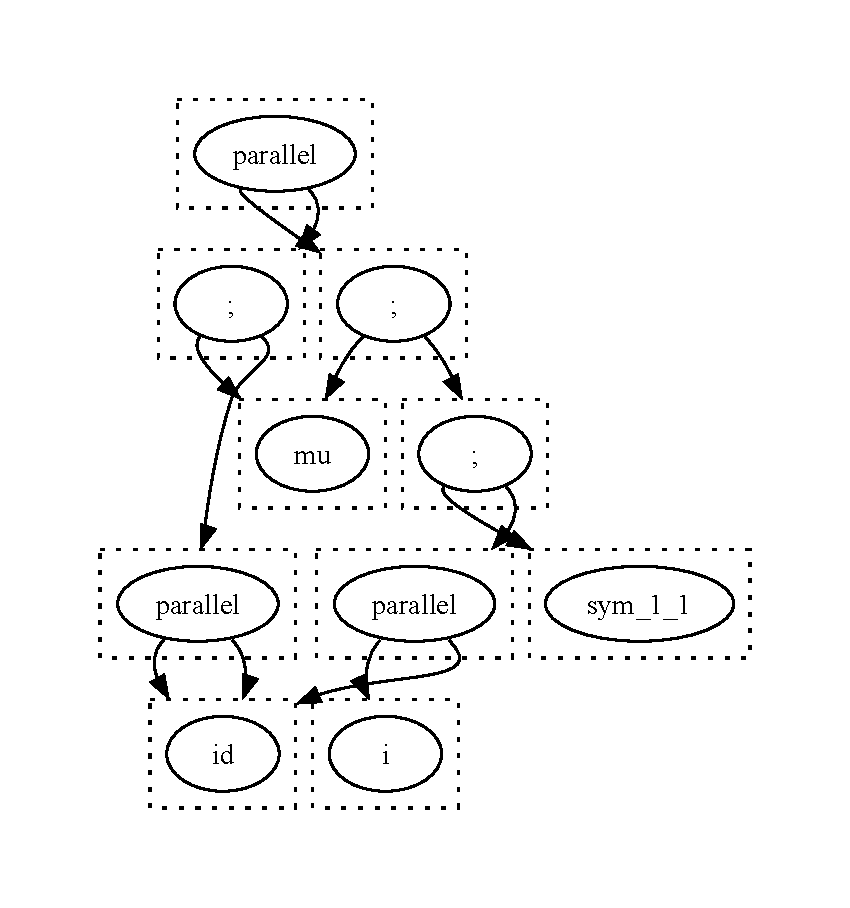
\includegraphics[scale=0.4]{figures/egraph_before_saturation_fix.pdf}
        \end{figure}
    \end{example}
\end{frame}

\begin{frame}
    \small
    \begin{example}
        \vspace{1em}
        E-graph for
        \[
            (\mu\;;(\sigma_{1,1}\;;i \otimes id_{1})) \otimes (\mu\;;(id_{1}\otimes id_{1}))
        \]
        After saturation
        \begin{figure}
            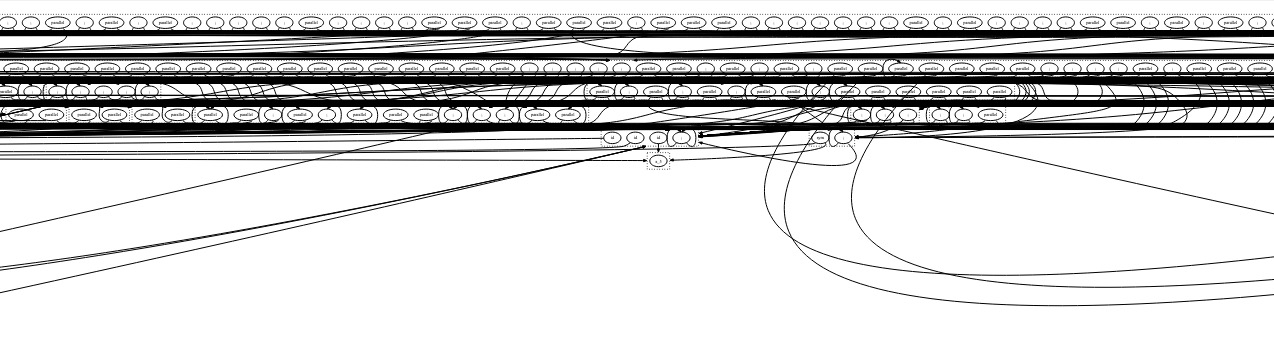
\includegraphics[width=0.9\linewidth]{figures/dot_5.jpeg}
        \end{figure}
        
        \end{example}
\end{frame}


% \begin{frame}
%     Another benefit of string diagrams is that they simplify the additional equations for which their term-equivalent form is not immediately obvious

%     \[
%          \scalebox{1}{
%             \tikzfig{figures/Z_spider_fusion}
%          }   
%     \]
% \end{frame}



% \begin{frame}{}
% \small
% The non-destructive feature of rewriting with e-graphs is modelled by using the idempotence property of $+$
% \vfill
% Given a rewrite rule (in a string diagrammatic form) and a source string diagram
% \begin{minipage}{0.4\linewidth}
%     \[
%     \scalebox{1}{
%     \tikzfig{figures/rewrite_example_1}
%     }
%     \]
% \end{minipage}
% \hfill
% \begin{minipage}{0.4\linewidth}
%     \[
%     \tikzfig{figures/rewrite_example_3}
%     \]
% \end{minipage}

% \end{frame}

% \begin{frame}
%     We apply the equations (and the rewrite rule above) in the following way
%     \[
%     \tikzfig{figures/rewrite_example_2}
%     \]
% \end{frame}


% \begin{frame}{}
%     Such extended string diagrams have a concrete combinatorial representation which we call \textit{e-hypergraphs} with interfaces


%         \begin{minipage}{0.45\linewidth}
%             \[
%             \tikzfig{figures/boxed_sym_string}    
%             \]
%         \end{minipage}
%         \begin{minipage}{0.05\linewidth}
%             \[
%                 \to
%             \]
%         \end{minipage}
%         \begin{minipage}{0.45\linewidth}
%             \[
%             \scalebox{0.5}{
%             \tikzfig{figures/extended_cospan_example}
%             }
%             \]
%         \end{minipage}
% \end{frame}

% \begin{frame}{}
%     \vfill
%     Now equivalence classes represent equivalent subgraphs rather than subtrees
%     \pause
%     \vfill
%     \pause
%     Such combinatorial structures are shown to be \textit{sound} and \textit{complete} for representing terms of enriched SMTs
%     \vfill
%     \pause
%     String diagrammatic reasoning becomes e-hypergraph rewriting
%     \vfill
%     \pause
%     The latter is defined as a \textit{double-pushout rewriting} which is a convenient framework to study properties of a rewriting system, e.g. confluence, applicability of parallel rewrites etc.
%     \vfill
%     \pause
%     Note that they absorb the laws of symmetric monoidal category but not the structural rules for $+$
% \end{frame}

% \section{Case Studies}

% \bsubsection{(acyclic) E-graphs are e-hypergraphs for Cartesian monoidal theories}

% \begin{frame}{}
%     If we consider an SMT with a copy and delete generators we get essentially an algebraic theory, the one for which e-graphs are designed

%     That is, if we consider the generators (the inputs flow from bottom to top to follow the e-graphs presentation)
%     \[
% 	\scalebox{0.7}{
%   	 \tikzfig{../figures/categorical-semantics/Cartesian-equipment}
% 	}
%     \]

%     and equations

%     \begin{minipage}{0.4\linewidth}
%         \[
%             \scalebox{0.55}{
%             \tikzfig{../figures/categorical-semantics/Cartesian-theory}	
%             }
%             \]
%     \end{minipage}
%     \hfill
%     \begin{minipage}{0.5\linewidth}
%         \[
%             \scalebox{0.55}{
%             \tikzfig{../figures/categorical-semantics/Cartesian-naturality}
%             }
%         \]
%     \end{minipage}


%     We can show that our construction is indeed a generalisation of e-graphs
% \end{frame}

% \begin{frame}{}
%     First, consider how an e-class gets translated into a string diagrammatic form

%     \begin{example}
%     \[
%     \tikzfig{figures/e-graphs-translation-2}
%     \]
%     \end{example}

%     A general translation can be drawn as follows
%     \[
%     \tikzfig{figures/e-graphs-translation}
%     \]
% \end{frame}

% \begin{frame}{}
%     \small
%     This way applying equations to an e-graph can be seen as e-hypergraph rewriting

%     \[
%     \scalebox{0.5}{
%     \tikzfig{figures/e-graphs-translation-3}
%     }
%     \]\footnote{[1]Willsey, M., Nandi, C., Remy Wang, Y., Flatt, O., Tatlock, Z., and Panchekha, P., “egg: Fast and Extensible Equality Saturation”, 2020.}
%     Can be rendered as
%     \[
%         % \hspace{1.3cm}
%         \scalebox{0.38}{
%         \tikzfig{../figures/categorical-semantics/egraph-translation-step-by-step-a-b}
%         }
%     \]
% \end{frame}

% \begin{frame}
%     \vfill
%     This serves as a sanity check for our construction, provides a categorical presentation of e-graphs and therefore a possible framework for reasoning about them in terms of e-hypergraph rewriting
%     \vfill
% \end{frame}

% \bsubsection{Support for binding}

% \begin{frame}{}
%     \small
%     \vfill
%     Lambda calculus is a model for a Cartesian Closed SMT and the benefits of using string diagrams for lambda calculus is that they are automatically quotiented by $\alpha$-equivalence (variables just become wires) and by linear substitution
%     \vfill
%     Compare the following

%     \begin{minipage}{0.3\linewidth}
%         \[
%         \scalebox{0.5}{
%         \tikzfig{figures/e-graphs-binding-example-plain}
%         }
%         \]
%     \end{minipage}
%     \hfill
%     \begin{minipage}{0.3\linewidth}
%         \[
%         \scalebox{0.5}{
%         \tikzfig{figures/e-graphs-binding-example-indices}
%         }
%         \]
%     \end{minipage}
%     \hfill
%     \begin{minipage}{0.3\linewidth}
%         \[
%         \scalebox{0.5}{
%         \tikzfig{figures/e-graphs-binding-string}
%         }
%         \]
%     \end{minipage}
%     \vfill
    
% \end{frame}

% \begin{frame}
%     \vfill
%     Thus we can represent e-graphs for lambda calculus with string diagrams for an enriched Cartesian Closed SMT
%     \vfill
% \end{frame}

% \begin{frame}
%     \[
%         % \hspace{1.3cm}
%         \scalebox{0.4}{
%         \tikzfig{../figures/categorical-semantics/e-graph-substitution}
%         }
%     \]
%     \tiny{[2]\href{https://pldi23.sigplan.org/details/egraphs-2023-papers/12/Optimizing-Beta-Reduction-in-E-Graphs}{Optimizing-Beta-Reduction-in-E-Graphs}}
%     \[
%         % \hspace{1.3cm}
%         \scalebox{0.35}{
%         \tikzfig{../figures/categorical-semantics/e-string-substitution-2}
%         }
%     \]
% \end{frame}

% \section{Conclusion}

% \begin{frame}{}
%     \begin{minipage}{0.65\linewidth}
%     \small
%     \vfill
%     \begin{itemize}
%         \item We have presented a generalisation of e-graphs for SMTs which could broaden the area of application of e-graphs to
%         \vfill
%         \begin{itemize}
%             \item Quantum processes
%             \vfill
%             \item Probabilistic programming
%             \vfill
%             \item Digital circuits
%         \end{itemize}
%         \vfill
%         \item It also has benefits for algebraic theories like lambda calculus
%         \vfill
%         \item As a bonus we have a framework for reasoning about e-graphs in terms of graph rewriting
%         \vfill
%         \item We \textbf{did not} study the implementation of e-hypergraphs as a data structure and the corresponding equality saturation procedure
%     \end{itemize}
% \end{minipage}
% \begin{minipage}{0.3\linewidth}
%     \small
%     
\includegraphics[width=\linewidth]{figures/arxiv_qr}
%     Link to a pre-print$\;\uparrow$\\

%     Email for collaboration:\\
%     \alert{\url{axt257@student.bham.ac.uk}}
% \end{minipage}
% \end{frame}

\end{document}